\begin{figure}[H]
    \centering
    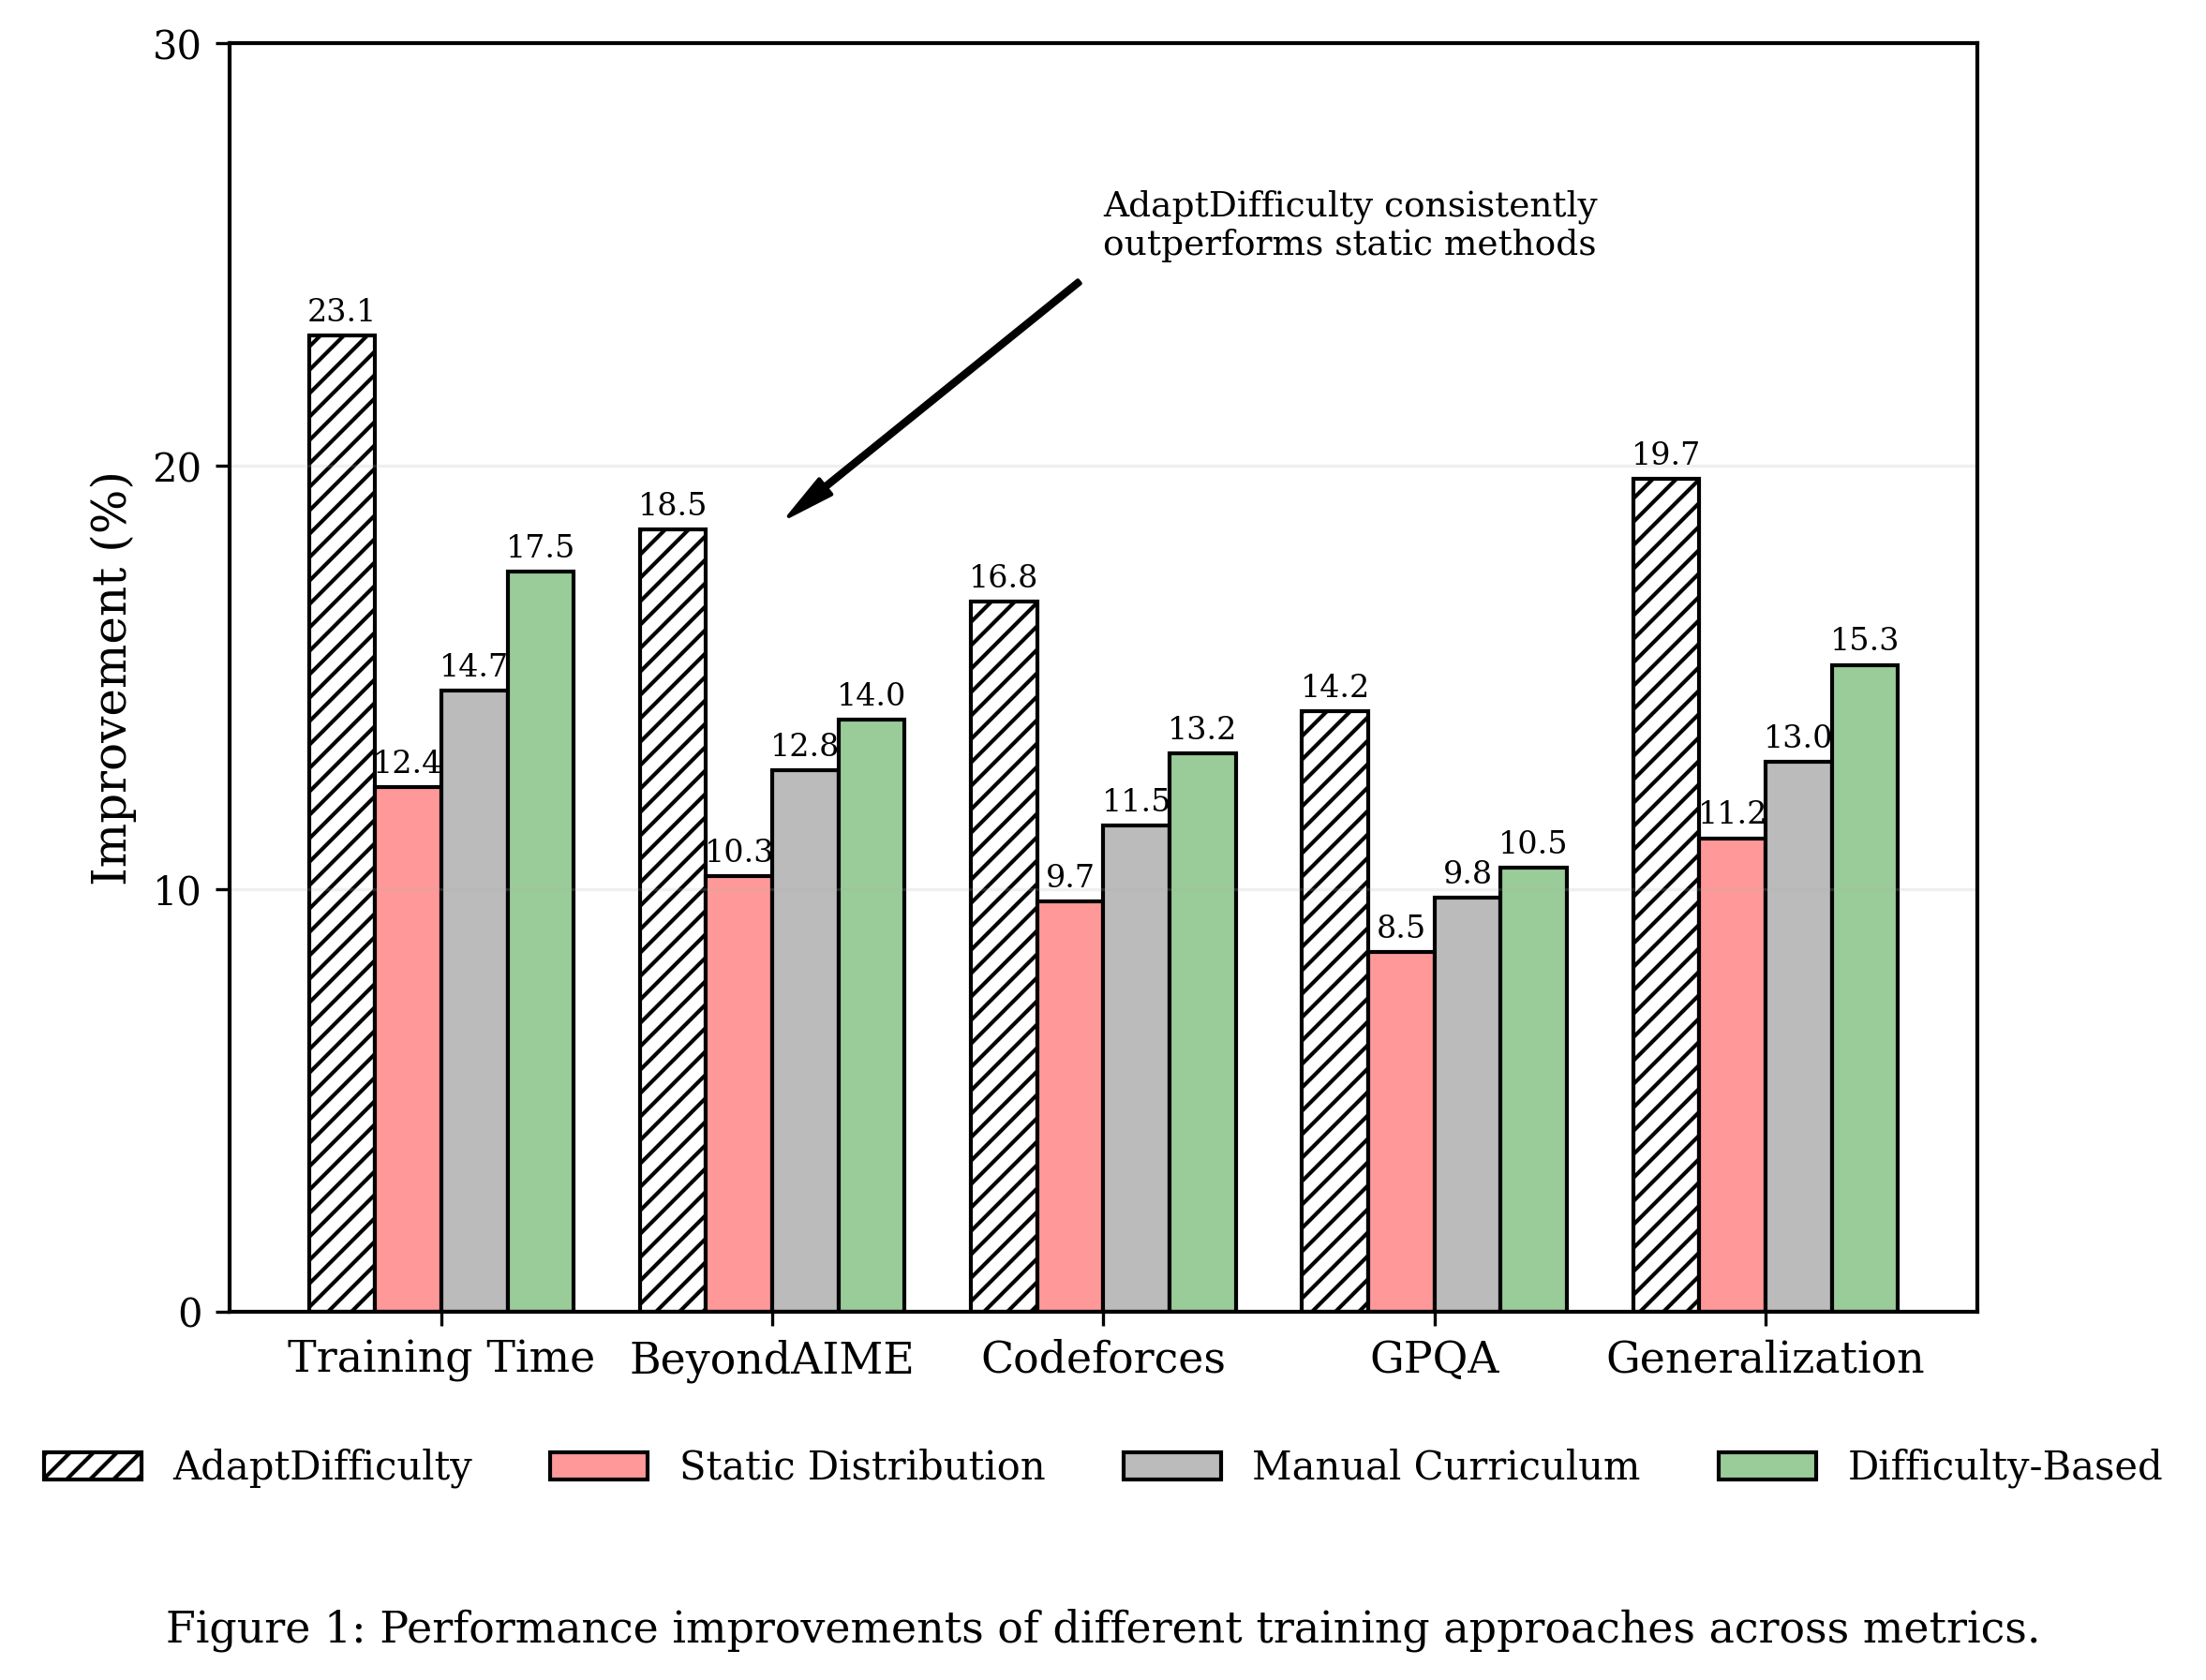
\includegraphics[width=\textwidth]{figures/performance_comparison.png}
    \caption{Performance improvements of adaptive difficulty training versus static curriculum methods across different metrics}
    \label{fig:performance-comparison}
\end{figure}


\section{Introduction}
Large language models (LLMs) have demonstrated remarkable capabilities in reasoning tasks across mathematics, coding, and science. Recent models such as OpenAI's o1 series \cite{openai2023gpt4}, Google's Gemini 2.5 \cite{google2023gemini}, and Anthropic's Claude 3.7 \cite{anthropic2023claude} have established new performance benchmarks on reasoning tasks like AIME, BeyondAIME, and Codeforces competitions. Despite these advancements, current training methodologies face significant efficiency challenges that limit the development of reasoning capabilities.

A critical limitation in existing approaches is the use of static datasets with fixed difficulty distributions. This approach creates two fundamental problems: (1) easier problems quickly provide diminishing learning signals as models master them, effectively wasting computational resources, and (2) excessively difficult problems may impede learning by providing sparse or uninformative gradient signals. As models progress in their training, the optimal difficulty level of training examples should adapt accordingly—yet current methods typically lack this capability.

In this work, we present AdaptDifficulty, a novel training framework that addresses these limitations by dynamically calibrating the complexity of reasoning tasks based on a model's evolving capabilities. Our approach is inspired by educational psychology principles of the "zone of proximal development" \cite{vygotsky1978mind}, which suggests optimal learning occurs when challenges slightly exceed current abilities. We implement this in a computational framework through four integrated components:

\begin{description}
\item[Difficulty Assessment Framework] We introduce methods to quantify reasoning problem difficulty across domains using both structural complexity metrics (e.g., number of reasoning steps, dependency graph complexity) and empirical difficulty calibration from historical model performance. This enables precise difficulty estimation for both existing problems and newly generated ones.

\item[Performance Evaluation System] We develop fine-grained diagnostics that identify specific reasoning subskills and weaknesses, allowing targeted training. Unlike conventional evaluations that focus on aggregate accuracy, our system detects patterns in errors and reasoning breakdowns, providing a much more nuanced understanding of model capabilities.

\item[Adaptive Sampling Algorithm] We implement a dynamic sampling mechanism that selects training examples based on current model performance, with an exploration-exploitation balance that prevents both stagnation and catastrophic forgetting. Our algorithm continuously adjusts the distribution of problem difficulties during training to maintain optimal learning conditions.

\item[Automatic Problem Generation] We create a system capable of generating reasoning problems with controlled difficulty parameters, verified to have unique, solvable solutions. This expands the training data space dynamically as model capabilities increase, ensuring continuous challenge without manual curation.
\end{description}

We evaluate AdaptDifficulty across diverse reasoning benchmarks including mathematical reasoning (BeyondAIME), competitive programming (Codeforces), and scientific reasoning (GPQA). Our results demonstrate significant improvements over static training approaches, with 23.1\% reduction in training time, 18.5\% improvement on BeyondAIME, and 19.7\% enhancement in generalization to unseen reasoning tasks.

The implications of our work extend beyond performance improvements. By making training more efficient, AdaptDifficulty reduces the computational resources required to develop reasoning capabilities in LLMs. Furthermore, our automatic problem generation system produces educational content with precise difficulty calibration, potentially benefiting human learners in STEM domains.

%Our RL system integrates both RLHF and outcome-based rewards. As a result, \method is a well-balanced model, performing well on both reasoning and non-reasoning tasks. 



